\chapter{Results and Discussion}
\section{Baseline performance of ammonia concentration and colour level forecasting models}

\begin{table}[!ht]
  \centering
  \caption{\label{tab:baseline-result}Baseline.}
  \begin{NiceTabular}{clcccc}
      \toprule
      Rank & Model-Dataset & Test loss & Improvement & test & test \\
      \midrule
      1  & LSTM-ew3 & 0.0379$\pm$0.0009 & 3.32\%  &LSTM-ew3 & 0.0379$\pm$0.0009 \\
      2  & LSTM-sg7 & 0.0379$\pm$0.0004 & 4.77\%  &LSTM-sg7 & 0.0379$\pm$0.0004 \\
      3  & LSTM-ew4 & 0.0380$\pm$0.0003 & 2.06\%  &LSTM-ew4 & 0.0380$\pm$0.0003 \\
      4  & GRU-ew3  & 0.0386$\pm$0.0004 & 1.53\%  &GRU-ew3  & 0.0386$\pm$0.0004 \\
      5  & LSTM-sg5 & 0.0387$\pm$0.0004 & 4.44\%  &LSTM-sg5 & 0.0387$\pm$0.0004 \\
      6  & LSTM-ew2 & 0.0389$\pm$0.0004 & 1.77\%  &LSTM-ew2 & 0.0389$\pm$0.0004 \\
      7  & GRU-sg7  & 0.0390$\pm$0.0009 & -1.30\% &GRU-sg7  & 0.0390$\pm$0.0009 \\
      8  & GRU-sg5  & 0.0392$\pm$0.0008 & 3.21\%  &GRU-sg5  & 0.0392$\pm$0.0008 \\
      9  & GRU-ew4  & 0.0394$\pm$0.0004 & -0.77\% &GRU-ew4  & 0.0394$\pm$0.0004 \\
      10 & GRU-sg9  & 0.0400$\pm$0.0010 & -4.44\% &GRU-sg9  & 0.0400$\pm$0.0010 \\
      11 & GRU-ew2  & 0.0402$\pm$0.0012 & -3.34\% &GRU-ew2  & 0.0402$\pm$0.0012 \\
      12 & LSTM-sg9 & 0.0409$\pm$0.0006 & -5.41\% &LSTM-sg9 & 0.0409$\pm$0.0006 \\
      13 & LSTM-obs & 0.0411$\pm$0.0007 & -4.05\% &LSTM-obs & 0.0411$\pm$0.0007 \\
      14 & RNN-sg5  & 0.0413$\pm$0.0009 & 0.48\%  &RNN-sg5  & 0.0413$\pm$0.0009 \\
      15 & RNN-sg7  & 0.0417$\pm$0.0007 & 1.42\%  &RNN-sg7  & 0.0417$\pm$0.0007 \\
      16 & GRU-obs  & 0.0420$\pm$0.0006 & -1.45\% &GRU-obs  & 0.0420$\pm$0.0006 \\
      17 & RNN-ew2  & 0.0424$\pm$0.0006 & -9.28\% &RNN-ew2  & 0.0424$\pm$0.0006 \\
      18 & RNN-ew3  & 0.0426$\pm$0.0003 & -3.90\% &RNN-ew3  & 0.0426$\pm$0.0003 \\
      19 & RNN-ew4  & 0.0427$\pm$0.0005 & -1.43\% &RNN-ew4  & 0.0427$\pm$0.0005 \\
      20 & RNN-obs  & 0.0437$\pm$0.0012 & -1.16\% &RNN-obs  & 0.0437$\pm$0.0012 \\
      \bottomrule
  \end{NiceTabular}
\end{table}

\begin{figure}[h]
  \centering
  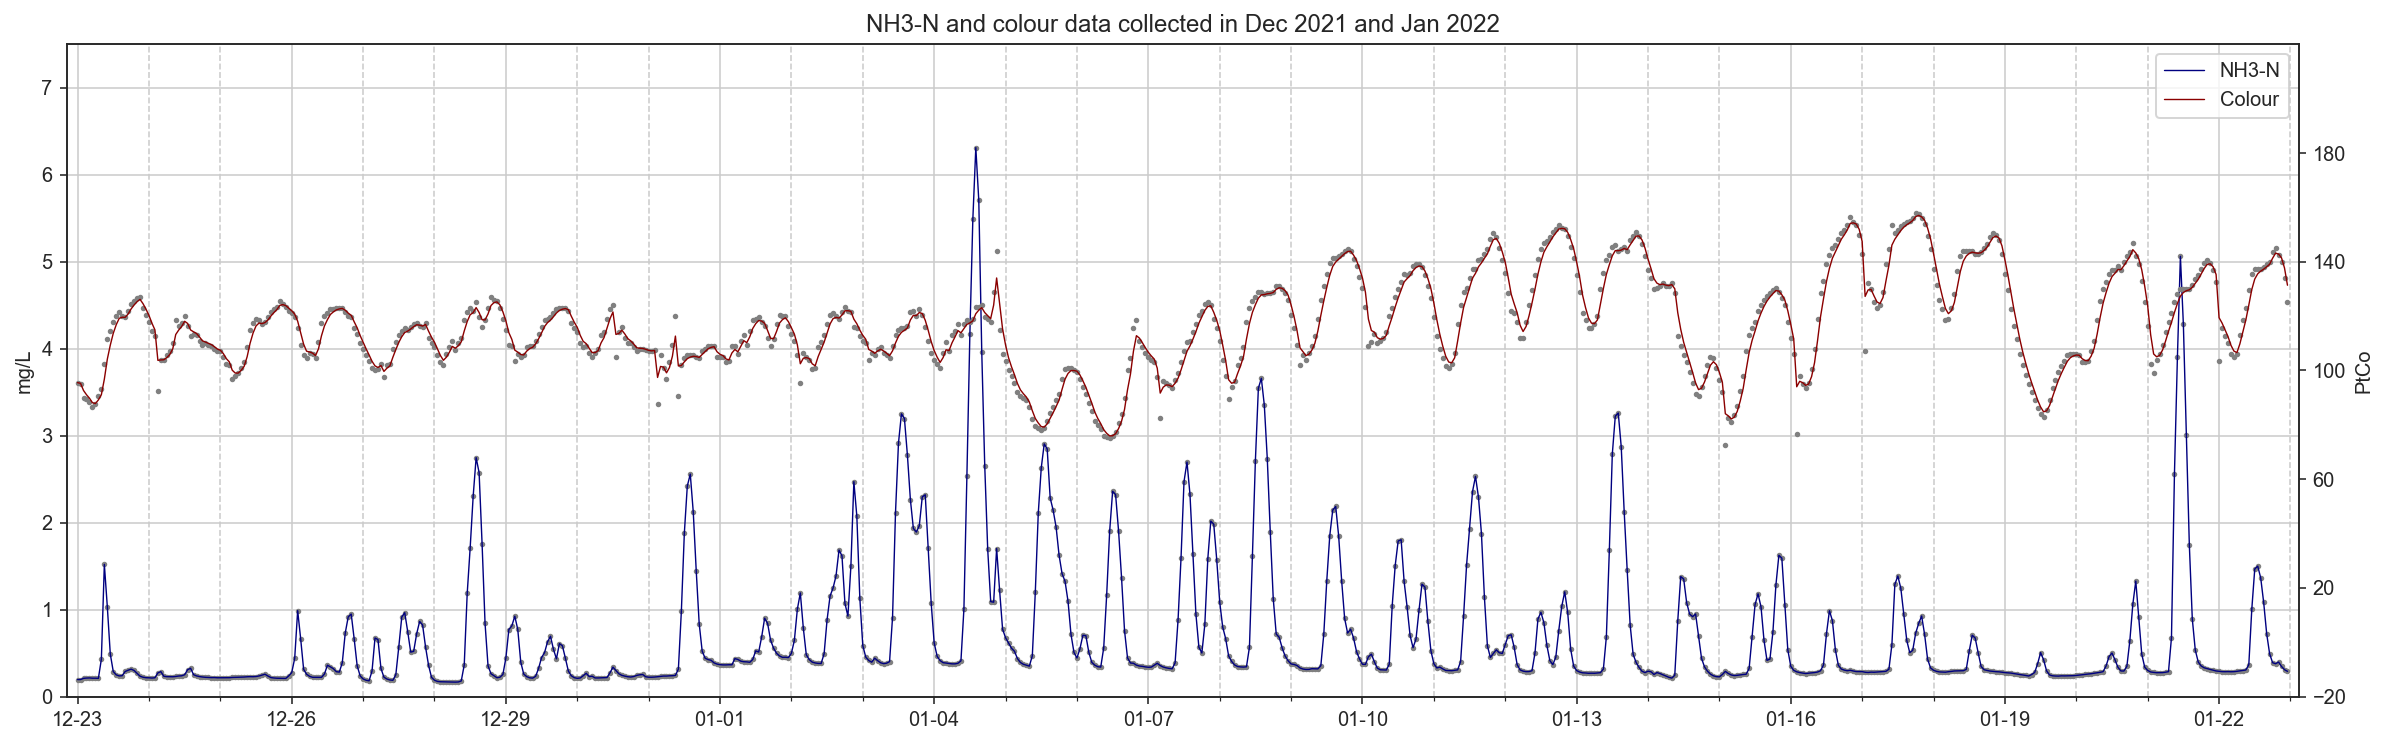
\includegraphics[width=1.0\columnwidth]{imgs/results/data.png}
  \caption{Ammonia and colour data collected from }
  \label{fig:nh3-color-data}
\end{figure}

\begin{figure}[h]
    \centering
    \begin{subfigure}{0.45\textwidth}
      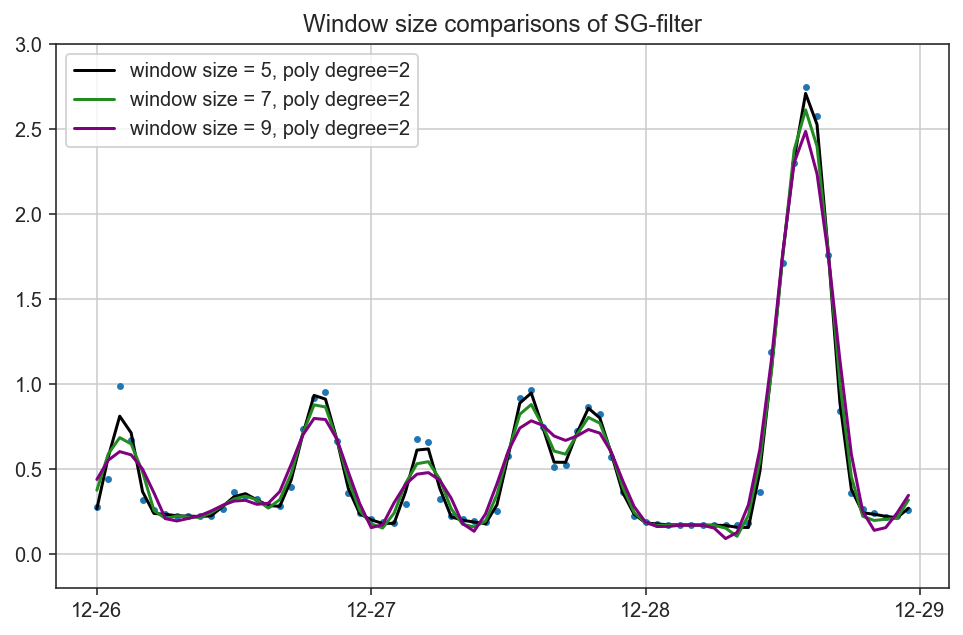
\includegraphics[width=\linewidth]{imgs/pre-processing/sg-filter.png}
      \caption{} \label{fig:smoothed-sg}
    \end{subfigure}%
    \hspace{2em}%   % maximize separation between the subfigures
    \begin{subfigure}{0.45\textwidth}
      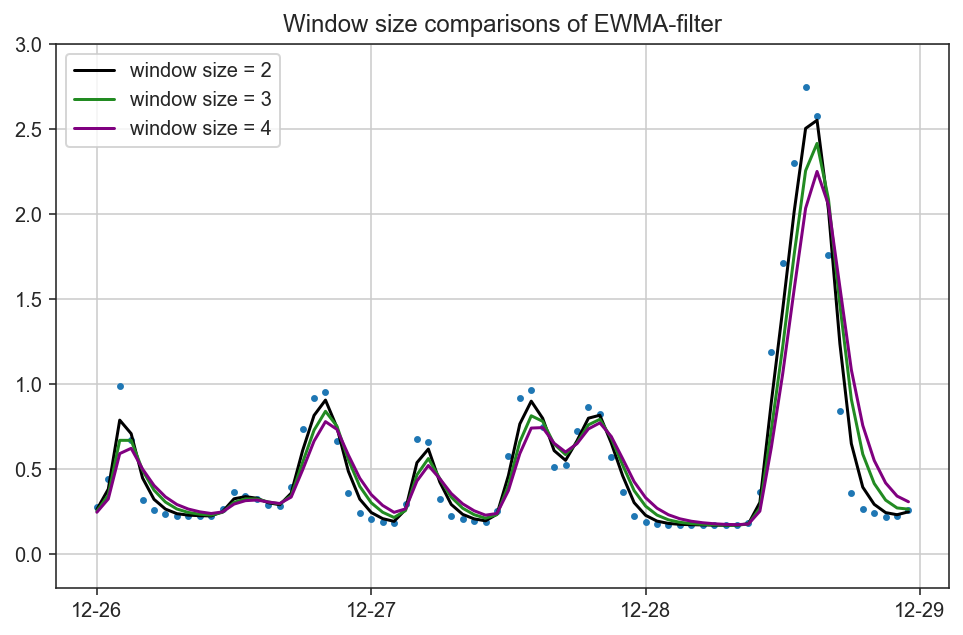
\includegraphics[width=\linewidth]{imgs/pre-processing/ew-filter.png}
      \caption{} \label{fig:smoothed-ew}
    \end{subfigure}%  
  \caption{Illustration of the influence of different polynomial degrees in the fitting of SG filter and the weigth decay with varied alpha values in EWMA filter.} \label{fig:smoothed}
\end{figure}
\subsection{Machine learning vs deep learning}
RF is used in this work as a representative tree-based modeling strategy because RF models have some major advantages over alternative tree-based models; notably, they require fewer hyperparameters for tuning, their performance is robust to hyperparameter changes, and they are less likely to suffer from overfitting (Breiman, 2001;Breiman, 2002 ;Chen and Guestrin, 2016;Fawagreh et al., 2014 ;Ke et al., 2017).
\section{Improved performance on forecasting models using data pre-processing techniques}
\section{Data enrichment via feature engineering based on effluent quality pattern}
\section{Design of model architecture through analyzing wastewater composition in sewer system}
